\chapter{Cluster Shape Encoding}
In this chapter my work will be discussed. First there will be a description of the data format, the cluster of pixels, analysing its properties and the reason behind the encoding. Then, a detailed description of the methods implemented will follow. Finally, the test of such methods will be reported.
\section{Cluster of Pixels}
\label{sec:cluster}
As said in the last chapter, the sensors of ITS-Upgrade are characterized by a binary readout and therefore only the information whether or not a particle was crossing the pixel is read out. Pixels in which the collected charge coming from the ionization exceeds a defined threshold are called \textit{fired pixels}. When a charged particle passes through a sensor, it loses energy in a region whose dimension depends on the parameters of the particle itself, such as its energy and the impact angle. Therefore normally it fires a set of adjacent pixels.\\
%
\begin{figure}
  \centering
  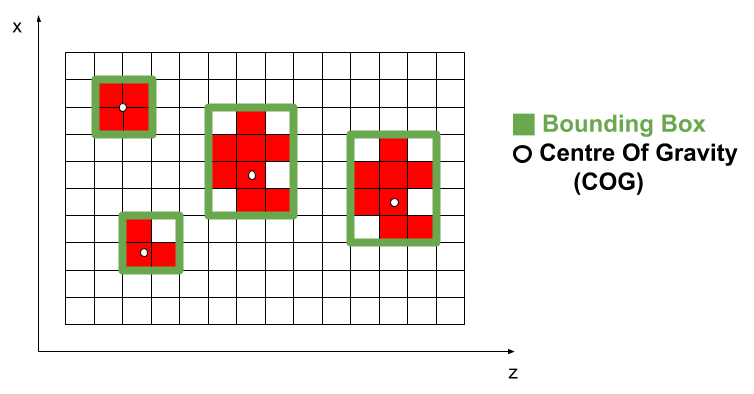
\includegraphics[scale=0.6]{figures/cluster.png}
  \caption{Example of different clusters on the same sensor. All the clusters have different positions, but two of them have the same shape.}
  \label{fig:clusters}
\end{figure}
%
A set of adjacent fired pixels forms a \textit{cluster}. Clusters are the data element of the ITS and are used for the reconstruction of the trajectories of the charged particles from which they have been generated. An example of clusters can be seen in Figure \ref{fig:clusters}. Each cluster in its raw format contains different kinds of information, which depend only on geometrical aspects. Each cluster has a particular shape, a specific pattern of fired pixels, which along my work is called \textit{topology}. As it can be seen in Figure \ref{fig:clusters}, different clusters can have the same topology.\\
Some characteristics are shared by clusters with the same topology. For example, the dimensions of the \textit{bounding box}, which is the smallest rectangle that can entirely contain the cluster, are clearly the same for all the clusters with the same shape. A second common piece of information is the position of the \textit{centre of gravity} (COG) of the topology within the bounding box, since this position is uniquely determined by the disposition of the fired pixels. The position of the COG is extremely important, since it is assumed to be the most probable impact position of the particle that generated the cluster. The uncertainty related to this quantity, which will be discussed later, is as well the same for all the clusters with the same topology.\\
The position of the cluster within the sensor is instead different from cluster to cluster. It is expressed as the coordinate of a reference pixel of the cluster within the matrix described by the pixels of the chip, in the form (\textit{row}, \textit{column}). The reference pixel of a cluster is defined as the pixel containing the COG of the cluster. This information is then converted into a physical length by a simple product of the coordinates by the pitch of the pixel. Each sensor has its own local frame, where z is the beam direction, x is orthogonal to z and lies on the surface of the sensor, y is orthogonal to the x-z plane, forming a right-handed Cartesian system. The passage from the local to the global frame is then performed during the reconstruction of the tracks, using matrices implemented in AliRoot.\\
In the next section the storage of the cluster data will be described, explaining the reasons behind this work.
\section{Data Compression}
The data size is an extremely important factor to hold in consideration during the design of a detector. The ALICE experiment, for example, has been designed for the study of heavy-ion collisions, with the necessity to identify all the particles produced in such collisions and to reconstruct their trajectories, and consequently a huge data volume is generated. As mentioned in section \ref{datavol}, after the trigger selection the data rate of all the detectors can reach 25 GB/s, while the physic content of many events could be small, with a DAQ archiving rate of about 1 GB/s. It is therefore clear that online processing is necessary to compress data avoiding the loss of physic content. The data rate will increase significantly after the upgrade, principally because of the higher collision rate. In particular, the data rate of all the detectors is estimated to be $\sim$ 1 TB/s \cite{o2}, where almost 1 TB/s is given by the TPC. For the ITS the data rate will increase both because of the higher collision rate and because of the higher number of readout channels ($\sim 10^{10}$). It is expected to be $\sim$ 40 GB/s, more than the current data rate of the whole ALICE apparatus. The data reduction starts immediately after the cluster-funding process and the information is compressed using Huffman coding, which will be shortly described in the next section. With Huffman compression it is possible to reduce the data size of a factor that depends on the the noise occupancy: in worst case scenario, with many noisy pixels, data size is reduced to  $\sim$ 26 GB/s, while in case of low noise it is reduced to $\sim$ 4.3 GB/s \cite{o2}.
\subsection{Huffman Coding}
\label{sec:huff}
Huffman coding is one of the most used lossless data compression algorithms, based on the relative frequency of the elements constituting a file. Huffman maps an element (for example a character in a text file) into a a bit sequence of variable length according to its frequency: the most frequent element is mapped into the shortest string. The result is a Huffman table, of which an example is given in Table\ref{tab:huff}. It is the Huffman table corresponding to the sentence ``\textit{Trentatrè trentini entrarono in Trento, tutti trentatrè trotterellando.}'': the most frequent character (t) is mapped into a two-bit sequence, while the least common ones are mapped in the longest bit strings. In this way it is possible to contain the information of the sentence in a shorter bit string. This example is trivial, but it allows to understand the utility of Huffman compression when applied to big files. Indeed, the most frequent character is encoded as the shortest bit string, therefore every time this character appears it is substituted by the corresponding Huffman code: the shortest string appears the highest number of times, allowing to save much storage space. Moreover, the less the frequency distribution of the elements is uniform, the more storage space is saved, since the most common character, hence the shortest bit string, appears much more often than the less common ones. This saving is obtained at the cost of creating a Huffman table and consulting it during the compression and the decompression processes, operations which are time consuming. For this reason, if the compression/decompression time is an important factor, it is necessary to pay attention to the number of entries in the table, since the former is proportional to the latter \cite{huffman}.
%
\begin{table}
\centering
 \begin{tabular}{|c|c|c|}
  \hline
  Character & Frequency & Huffman code\\
  \hline
  t & 15 & 01 \\
  r & 10 & 110 \\
  n & 9 & 101 \\
  e & 7 & 000 \\
  \_ & 7 & 001\\
  o & 5 & 1001 \\
  i & 4 & 11111 \\
  a & 3 & 11110 \\
  è & 2 & 10000 \\
  l & 2 & 10001 \\
  T & 2 & 111011 \\
  u & 1 & 111010 \\
  , & 1 & 111001 \\
  . & 1 & 111000 \\
  \hline
 \end{tabular}
 \caption{Huffman table related to the sentence ``\textit{Trentatrè trentini entrarono in Trento, tutti trentatrè trotterellando.}''.}
 \label{tab:huff}
\end{table}
%
\section{Cluster Data Encoding}
Every cluster is identified by its position and its topology. In section \ref{sec:cluster} it was said that the position of the cluster can be expressed as the coordinates of the reference pixel of the cluster within the sensor. This information must be combined with an identifier of the chip, whose position in the experiment frame is known. It is possible to store the position of the reference pixel not as its absolute raw number, but as the difference between its row number and that of the previous stored pixel. Studying the frequency distributions of these deltas, it can be seen that it is not uniform and consequently it is possible to benefit from this non uniformity using Huffman coding. Similarly, the identifiers of the chips can be stored as the difference between the identifier of the chip which is being analysed and the previous one. Its distribution is not uniform as well and this element can be compressed using Huffman too. Both this distributions are strongly dependent on the occupancy in the detector. For this reason it is possible to use different Huffman tables according to the multiplicity. In particular the multiplicity can be binned and for each multiplicity bin a Huffman table is defined. This information, together with the topology, defines the cluster data:
\begin{displaymath}
\begin{split}
  \mathrm{MultID[\textcolor{red}{\Delta ChipID_1}(\textcolor{Cerulean}{Col}, \textcolor{LimeGreen}{\Delta Row}, \textcolor{Plum}{Patt})_1 \  ... \ (\textcolor{Cerulean}{Col}, \textcolor{LimeGreen}{\Delta Row}, \textcolor{Plum}{Patt})_n \textcolor{SkyBlue}{\Delta EndChip}] }\\
 \mathrm{[\textcolor{red}{\Delta ChipID_2}(\textcolor{Cerulean}{Col}, \textcolor{LimeGreen}{\Delta Row}, \textcolor{Plum}{Patt})_1 \  ... \ (\textcolor{Cerulean}{Col}, \textcolor{LimeGreen}{\Delta Row}, \textcolor{Plum}{Patt})_n \textcolor{SkyBlue}{\Delta EndChip}]\ ...}
 \end{split}
\end{displaymath}
\textit{MultID} is the multiplicity bin, used to pick up the appropriate Huffman table to encode/decode the information about the row number and the identifier of the chip; \textit{$\Delta$ChipID} is the difference between the identifier of the cluster being analysed and the previous one; \textit{Col} is the column number of the reference pixel; \textit{$\Delta$Row} is the difference between the row number of the reference pixel of the current cluster and the previous one. \textit{EndChip} is a special identifier that flags the end of the chip. \textit{Patt} is instead the information related to the topology, which will be discussed in the next section.
\section{Cluster Topology Encoding}
The cluster topology, in its raw format, consists of a sequence of bits whose length depends on the number of pixels within the bounding box: a fired pixel is represented by a 1, while an off one by a 0. Such a string can become very long for large clusters, therefore storing the information about the cluster topology as the complete bit-mask would require the usage of much storage space.
%
\begin{figure}
  \centering
  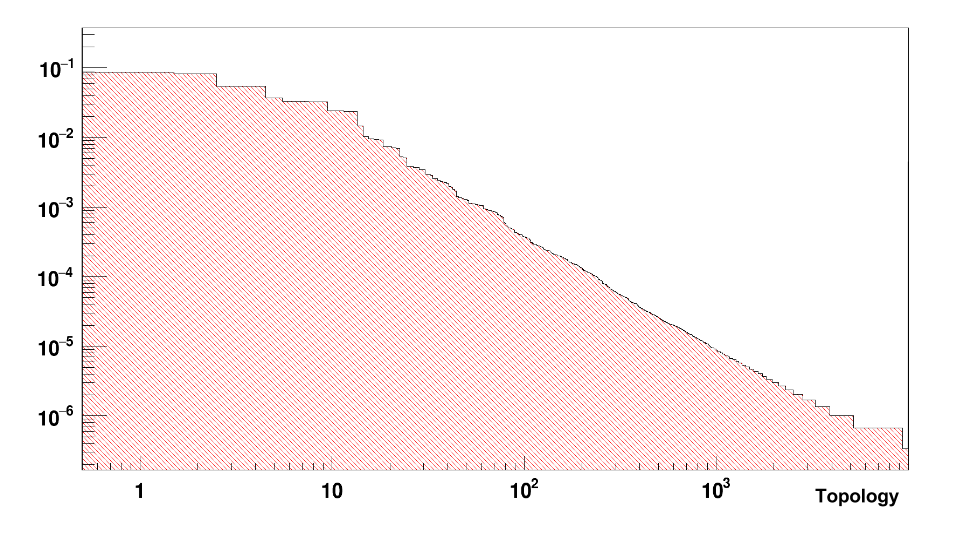
\includegraphics[scale=0.4]{figures/topdistro.png}
  \caption{Frequency distribution of the topologies obtained through a Monte Carlo simulation of 20 Pb-Pb events.}
  \label{fig:topdistro}
\end{figure}
%
This issue can be solved creating a dictionary containing all the topologies. In this way it is possible to store a reference to an entry of the dictionary instead of the complete bit-mask. Since a reference is an integer, its length is fixed. In Figure \ref{fig:topdistro} a frequency distribution of the topologies, obtained simulating 20 minimum-bias Pb-Pb events, is reported. This distribution is highly non uniform and consequently the compression via Huffman would be extremely convenient in terms of storage space. However, due to the high number of different elements, the processes of compression and decompression become inefficient. Therefore, there is the necessity to reduce the number of entries in the dictionary and this can be done grouping rare topologies, whose frequency is under a defined threshold, under a common reference.\\
In the next sections the steps to the construction of the dictionary of the topologies will be described and a detailed description about the method of grouping will be given.
\section{Software Development}
The objective of this work is the implementation of some software for the construction of the dictionary and for the realisation of the related mechanisms of matching between the cluster topology the corresponding entry in the dictionary. In particular this software will be used online, during the data acquisition in Run3. It must not be developed to work in AliRoot or ROOT environment: the two data analysis frameworks contain many features that are not necessary during the data acquisition and therefore the machines used for online operations have nor AliRoot and ROOT installed. For this reason several C++ classes, which can be used on every machine with a C++ compiler installed, have been implemented:
\begin{itemize}
 \item \textbf{MinimTopology} is a support class which contains the whole information necessary to characterize a topology;
 \item \textbf{Dictionary} is the proper dictionary, containing the information about all the common topologies and the groups of rare topologies;
 \item \textbf{BuildDictionary} is the class dedicated to the construction of the dictionary starting from the data;
 \item \textbf{LookUp} is used to match online the topology of clusters with the corresponding entry in the dictionary;
 \item \textbf{FastSimulation} can simulate a population of topologies with a frequency distribution determined by the dictionary. 
\end{itemize}
\section{Uniqueness of the Keys in the Dictionary: Hash Functions}
The dictionary must fulfill few requirements. First of all, each entry in the dictionary must be uniquely identified by a key. The key must have specific characteristics: it must have a defined length, which must be the same for each entry of the dictionary, and it must be comparable with the other keys, in order to be sortable. Typically in a database the key is an integer, since such a type has the needed characteristics. Unfortunately the topology is a bit string whose length is determined by the size of the bounding box and it cannot be used as a key. It is necessary to convert the topology as a string of variable length into a string of defined length. This operation is performed using a \textit{hash function}, which is a function that maps data of arbitrary size into data of fixed size. In particular in this work a C++ implementation of the function MurmurHash2 is used. The name suggests its working principle, since it is the combination of the words multiply (Mu) and rotate (r): MurmurHash2 processes the input string four bytes at a time, performing bitwise and multiplication operations, and combines all the four-byte chunks to give as a result a four-byte sequence. The choice of MurmurHash2 was made considering its characteristics: it has a good uniformity of the output distribution and is fast if compared with other algorithms \cite{hash}. Indeed, the hash function must be as fast as possible, since it must be used online. The uniformity of the output instead is related to the non injectivity of the hush function: while the input of the hash function can be any string of bits, the output must be a positive integer (four-byte sequence) and therefore can be each integer in the range [0, 2$^{32}$ - 1]. If the distribution of the outputs is uniform, then its more likely that two different input strings are mapped into two different integers. Unfortunately, even if the MurmurHash2 function has a good uniformity, it is not injective: in very rare cases (< 1/1000) two different strings are mapped into the same hashcode. All the classes must be solved to use the dictionary: this operation is done in the class \textit{MinimTopology}, which will be described in the next section.
%
\begin{figure}
  \centering
  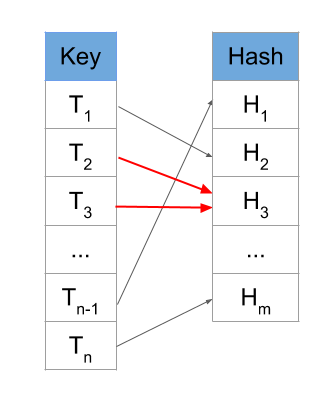
\includegraphics[scale=0.5]{figures/clash.png}
  \caption{Example of clash: MurmurHash2 maps two topologies (T$_2$ and T$_3$) into the same hashcode (H$_3$).}
  \label{fig:clash}
\end{figure}
%
\section{Class MinimTopology}
The class MinimTopology is the basis of this work since it is used by all the other classes. This class contains the information necessary to characterize a topology: the pattern, in string format, and the corresponding hashcode, generated from the first with a method that will be described soon. Starting from the pattern, the only sequence of bits is not enough to identify uniquely. For example, the sequence 1111 could represent four fired pixels in a raw, or four fire pixels in a column, or a square of four pixels, all fired. Beside this information also the dimensions of the bounding box are needed. In this way it is possible to correctly interpret the sequence of pixels that constitutes the pattern. An example of pattern encoding within the class MinimTopology is given in Figure \ref{fig:pattern}. This topology has three rows and three columns, corresponding to a sequence of nine pixels. The pattern is encoded in a string where the first two bytes are respectively the number of rows and the number of columns. The remaining bytes of the string are used to encode the proper pattern, i.e. the sequence of pixels that constitutes the topology itself. In the example the pattern consists of nine pixels, therefore two bytes are necessary, since a byte is made of 8 bits. A 1 is associated to each fired pixel, a 0 to each off one. From this string a four-byte hashcode is generated using MurmurHash2, but at this stage it is possible that two different patterns are mapped into the same 4-byte sequence. There is therefore the necessity to solve the clashes. One method could be to mark with a flag the entries of the dictionary for which there is a clash and then proceed with the direct comparison between the patterns until the ambiguity is erased. However this method require additional operations: first it is necessary to check whether the hashcode is marked with a clash-flag (even if there are not collisions) and then to resolve the ambiguities through a direct comparison. In fact there is a method to avoid the useless operation of the flag check: it is possible to use a eight-byte hashcode, in which the first four bytes are the usual four-byte hashcode previously described and the last four bytes are the first four byte which constitutes the pattern (the bytes starting from the third one of the string). In this way when two eight-byte hashcodes are compared it is performed both a comparison of the hash generated with MurmurHash2 and of the first 32 pixels, so that in case two different topologies are mapped into the same four-byte sequence by the hash function the clash is solved at the same time of the four-byte hashcode comparison.
\begin{figure}
  \centering
  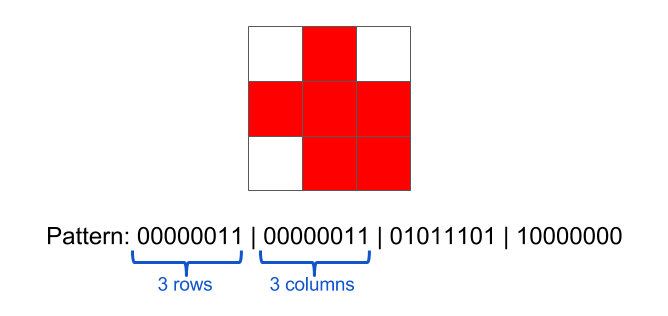
\includegraphics[scale=0.5]{figures/pattern.png}
  \caption{Example of pattern encoding: the first two bytes are respectively the number of rows and the number of columns; the remaining bytes are the pattern itself.}
  \label{fig:pattern}
\end{figure}
%
Summing up, the class MinimTopology has two data members:
\begin{enumerate}
 \item a string in which the pattern of pixels is stores;
 \item a eight-byte hashcode, generated from the pattern with the method just described, which uniquely identifies the topology.
\end{enumerate}
%
\section{Reduction of the Entries of the Dictionary: Grouping}
The second requirement for the dictionary concerns the number of entries. As said in section \ref{sec:huff}, the Huffman becomes inefficient when the number of different elements (in this case the number of topologies within the dictionary) is high. For this reason there is the necessity to limit the number of entries of the dictionary to at most O(10$^3$). This objective is achieved grouping rare topologies under a common reference, called \textit{GroupID}. The groups must be formed to gather rare topologies with similar characteristics, i.e. with similar errors related to the estimated impact position of the particle that generated the cluster. The grouping is necessary a lossy operation, since the information about the pattern of pixels, and therefore about the position of the impact point of the single rare topology, is lost in favour of average quantities. However this loss is bearable, since it concerns rare topologies and therefore it interests a very small fraction of the data.\\
The chosen grouping criterium concerns the dimensions of the bounding box: it is based on the assumption that topologies with similar dimensions have similar uncertainties related to the impact point position. As it will be seen later, for each topology the uncertainty on the impact point position is get from the distribution of the impact points themselves (or rather their first reconstruction) with respect to the COG position. In the case of groups of rare topologies this method is not applicable, since in different topologies the position of the COG within the bounding box can be extremely different and the distribution of the impact points (their first reconstruction) can be different too. Since it is not possible to rely on these distributions, the error is evaluated with the most pessimistic method: the position of the COG is assumed to be equally probable in the whole area of the bounding box. The error associated to the position of the COG is therefore that of a uniform distribution. In particular, a uniform distribution in the range of x(z) dimension of the bounding box:
\begin{equation}
 \sigma_x \; = \; \frac{N_{rows} \cdot d_x}{\sqrt{12}} \ \ \ \ \  \sigma_z \; = \; \frac{N_{columns} \cdot d_z}{\sqrt{12}}
\end{equation}
Considering a uniform distribution maybe the error is a bit overestimated, but it must be considered that this approximation involves rare topologies and hence a very small fraction of the data.\\
The grouping is based on a two-dimensional binning: a rare topology is assigned to a particular group according to its number of columns and rows. An example of grouping can be seen in Figure \ref{fig:gruppi}.

\begin{figure}
  \centering
  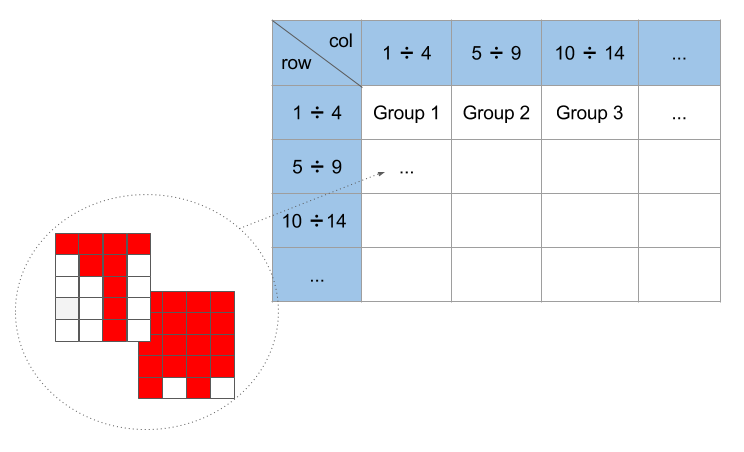
\includegraphics[scale=0.5]{figures/gruppi.png}
  \caption{Example of grouping: the two rare topologies have the same number of rows and columns and belong to the same group.}
  \label{fig:gruppi}
\end{figure}
%